\chapter[Hyperparameters]{Hyperparameters}
\label{ch:Hyperparameters}

\index{Hyperparameters|(}
\cite{Li2017} state that `performance of machine learning algorithms depends critically on identifying a good set of hyperparameters'. Hyperparameter tuning is a topic often discussed in literature describing any combination of machine learning algorithms. Adequate values set for hyperparameters will massively influence training and testing of a model, be it in terms of processing time, as well as the actual robustness of the model in question. 

\section{Introduction}\label{sec:introduction}
\subsection{Defining Hyperparameters}
\label{sec:defining-hyperparams}

As explained by \cite{Bergstra2012}, consider a learning model $A$ attempts to map a set of training data $X_{train}$ to a function $f$ which minimizes generalization loss. The model has a set of parameters which may be optimized during training, which are referred to as \textit{model parameters}. The learning algorithm also has a set of parameters which define its architecture and how the system will behave. These may not be changed at runtime, and are referred to as \textit{hyperparameters}. The training and testing performance of a function in relation to minimizing validation error depends heavily on selecting appropriate hyperparameter configurations.


\section{Approaches for Hyperparameter Optimization}\index{Hyperparameter Optimization}
\label{sec:optimization-approaches}
Various methods exist to find optimal hyperparameter sets. A multitude of published works go into methods such as \textit{grid search}, where one may refer to \cite{Duan2005}. \textit{Random search} is another approach, explored in detail by \cite{Bergstra2012}. Other approaches make use of \textit{Bayesian Optimizations}, such as \cite{Snoek2012} and \cite{Snoek2015}. \textit{Gradient-Based} methods have also been used for hyperparameter tuning, in works such as \cite{SathiyaKeerthi2006}. An overview and comparison of a number of these approaches will be provided in the sections to follow.


\subsection{Grid Search vs. Random Search}\index{Grid Search, Random Search}
\label{sec:grid-search-vs-random-search}
Two common approaches for tuning hyperparameters are grid search and random search. Grid search is an exhaustive method which will go through every possible combination of a set of hyperparameters, similarly to a brute-force methodology. The hyperparameter set with the best results is then kept and used for the model. Figure \ref{fig:grid_search} shows grid search being applied on a  system consisting of two hyperparameters.

\begin{figure}
	\centering
	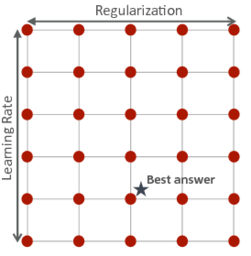
\includegraphics[width=0.45\linewidth]{graphics/hyperparameters/grid}
	\caption{Grid search on a 2D hyperparameter space, adapted from \url{http://prog3.com/sbdm/blog/google19890102/article/details/50276693} and \url{researchgate.net}}
	\label{fig:grid_search}
\end{figure}

By observing Figure \ref{fig:grid_search}, it is clear that grid search is guaranteed to find a correct answer due to its exhaustive nature. In order to compare this method with a different approach, \cite{Bergstra2012} conducted a study to compare randomly sampled hyperparameters with those obtained through a grid search. Here they refer to a set of model coefficients $\theta$ and hyperparameters $\lambda$. As stated previously, the objective for a learning algorithm is to find the $\lambda$ which minimizes a loss function $f$.  Figure \ref{fig:random_search} shows random search working within the same space as the previous image.


\begin{figure}
	\centering
	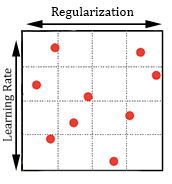
\includegraphics[width=0.5\linewidth]{graphics/hyperparameters/random}
	\caption{Random search on a 2D hyperparameter space, image adapted from Figure \ref{fig:grid_search}}
	\label{fig:random_search}
\end{figure}


\noindent Weighing both approaches together, random search could land on the best answer in the first trial, or the last. Consider the following example:\\

An SVM has several hyperparameters, one may consider $\gamma$, $C$, and the kernel type for the sake of this example. $\gamma$ defines the influence of observations on the model, $C$ affects the strictness of classification, and the kernel will affect the shape of the SVM's decision boundary.\\\\

These may be represented as follows:

\[kernel = [linear, polynomial, RBF] \]

\[\gamma = [0.0001, 0.001, 0.01, 0.1 , 0.5, 1, 1.5]\]

\[C = [0.001, 0.01, 0.1, 1, 1.5] \]

For this very simple example, grid search would take $3*7*5 = 105$ runs of an SVM to check each and every hyperparameter combination. With random search, there is a possibility to discover a good configuration much faster, perhaps even instantly. This is particularly the case in real life examples where there may be many more hyperparameters than the ones presented.  Since grid search makes use of every possible combination, the system suffers from the \textit{curse of dimensionality}, described by \cite{Chen2009} and \cite{Bellman2015}. This results in the algorithm complexity growing exponentially as the number of hyperparameters increase. This constrains grid search to being competitive only in lower dimensional spaces.\\

Thus, once a problem exceeds two hyperparameters, and sometimes even with only two, random search becomes vastly more efficient according to \cite{Bergstra2012}. Nevertheless, many studies such as \cite{Duan2005,E.Hinton2010} and machine learning libraries such as \textit{libsvm} by \cite{Chang2011}, employed a combination of grid search and manual search\index{manual search}. Knowing this, Bergstra and Bengio showed that random search actually generally outperforms grid search for hyperparameter optimization. This is true even when taking into account the element of luck required by random search, since hyperparameter trials are randomly sampled without any selection criteria. \cite{Snoek2012} states that this property provides random search yet another advantage grid search, since the algorithm can operate without caring about which hyperparameters are important to the model.


\subsection{Bayesian Optimization of Hyperparameters}\index{Bayesian-Optimization}
\label{sec:bayesian-optimization}
\cite{Press2005} defined Bayesian techniques as methods making use of Bayes' theorem\index{Bayes' theorem} to combine observational data with subjective beliefs.  Bayes' theorem states that considering a hypothesis $H$ and evidence $E$, the probability of $H$ happening given that $E$ has occurred is calculated as follows:

\[P(H|E) = \frac{P(E|H)P(H)}{P(E)}\]

Bayesian optimizations provide a reasonable approach to modelling uncertainty. According to \cite{Snoek2015}, they also provide a natural framework for optimizations of expensive black-box functions.Returning to the scope of hyperparameter tuning, one may consider a hypothesis as a set of hyperparameters $\lambda$ and the evidence as data $D$. Bayesian approaches will keep $D$ static, and modify hyperparameter configurations $\lambda$ instead to see how the output changes. Essentially, the resulting data obtained through a certain hyperparameter set is then used to predict an expectation for different hyperparameter values. This may be repeated until convergence to a local optimum is reached. Regarding performance, \cite{Snoek2012} compared Bayesian approaches to an exhaustive grid search for optimizing hyperparameters of M3E models with three hyperparameters. The conclusion of the study was that the Bayesian approach was reasonably more efficient than grid search. This also makes sense 

\subsection{Gradient-Based Hyperparameter Optimization}\index{gradient-descent}
\label{sec:gradient-based-optimization}
A particular project by \cite{SathiyaKeerthi2006} investigates hyperparameter values in SVMs and Bayesian models. In this system, the variables $C$ and $\gamma$ are considered. $C$ is the regularization coefficient, influencing how leniently the SVM hyperplane classifies observations. Figure \ref{fig:smallc} and Figure \ref{fig:bigc} show how different values of $C$ influence a decision space for classification.

\begin{marginfigure}%
	\centering
	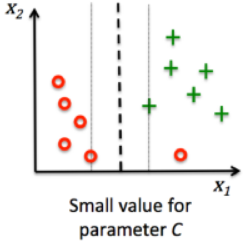
\includegraphics[width=0.8\linewidth]{graphics/hyperparameters/small_c.png}
	\caption{Small $C$}
	\label{fig:smallc}
\end{marginfigure}
\begin{marginfigure}%
	\centering
	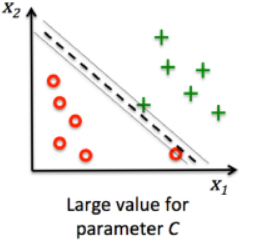
\includegraphics[width=0.8\linewidth]{graphics/hyperparameters/big_c.png}
	\caption{Big $C$, both images from \url{https://www.bogotobogo.com/python/scikit-learn/scikit_machine_learning_Support_Vector_Machines_SVM.php}}
	\label{fig:bigc}
\end{marginfigure}

 As previously stated, $\gamma$ defines the influence of points on the variance of a model.  As expected, experiments in this study showed that performance of the SVM varied considerably as a function of hyperparameter values. Gradient-based optimization techniques were used, computing the slope of a performance validation function with respect to the vector $h$ of hyperparameters. The gradient-descent approach attempts to minimize the cost function of the hyperparameter problem by converging to local minima. To reach this goal, the gradient of the function decreases with each iteration of the algorithm. This will update the  coefficients $\beta$ of the system, which will then be applied to the feature vectors in the next iteration. This process is repeated until convergence towards a local minimum is reached. This system allowed for a fast method to determine optimal sets of hyperparameters, which also outperformed grid search even for models with a low dimensionality of two hyperparameters.

\index{Hyperparameters|)}